\setlength{\columnsep}{3pt}
\begin{flushleft}
Classful addressing:
\begin{itemize}
		\item Was introduced in 1981
		\item Divides the IP address into five separate classes:
		\begin{itemize}
			\item Class A
			\item Class B
			\item Class C
			\item Class D
			\item Class E
		\end{itemize}
		\item Below image shows the details of each class in detail:
		\begin{figure}[h!]
			\centering
			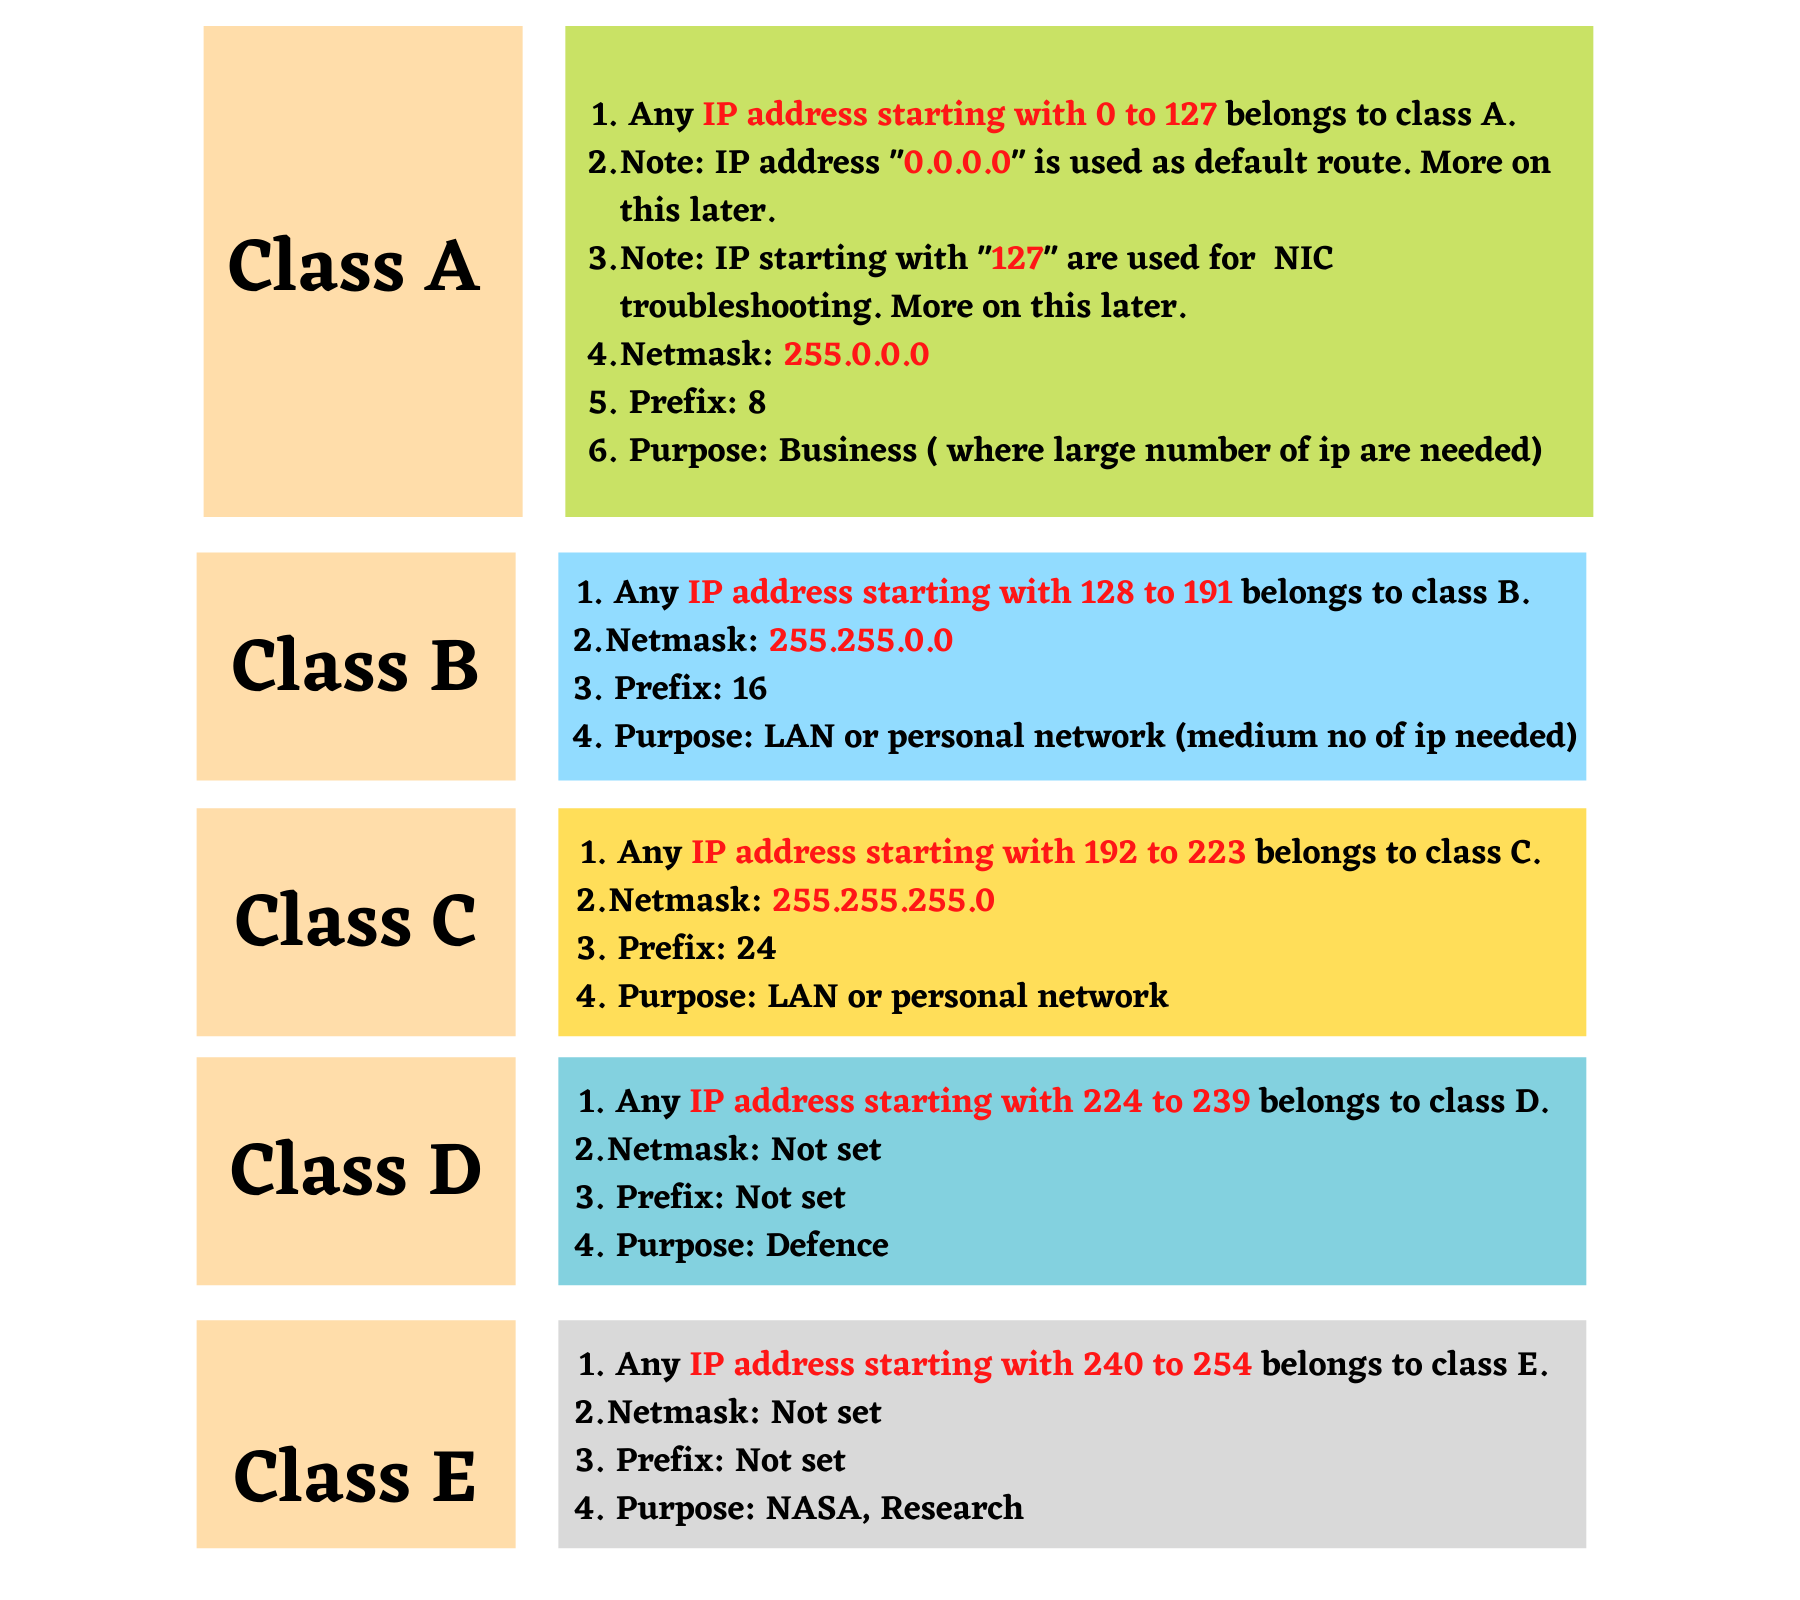
\includegraphics[scale=.3]{content/chapter14/images/ip_classes.png}
			\caption{IP address classes}
			\label{fig:type}
		\end{figure}	
\end{itemize}

\newpage
\paragraph{Example of IP address and their class:}
\begin{figure}[h!]
	\centering
	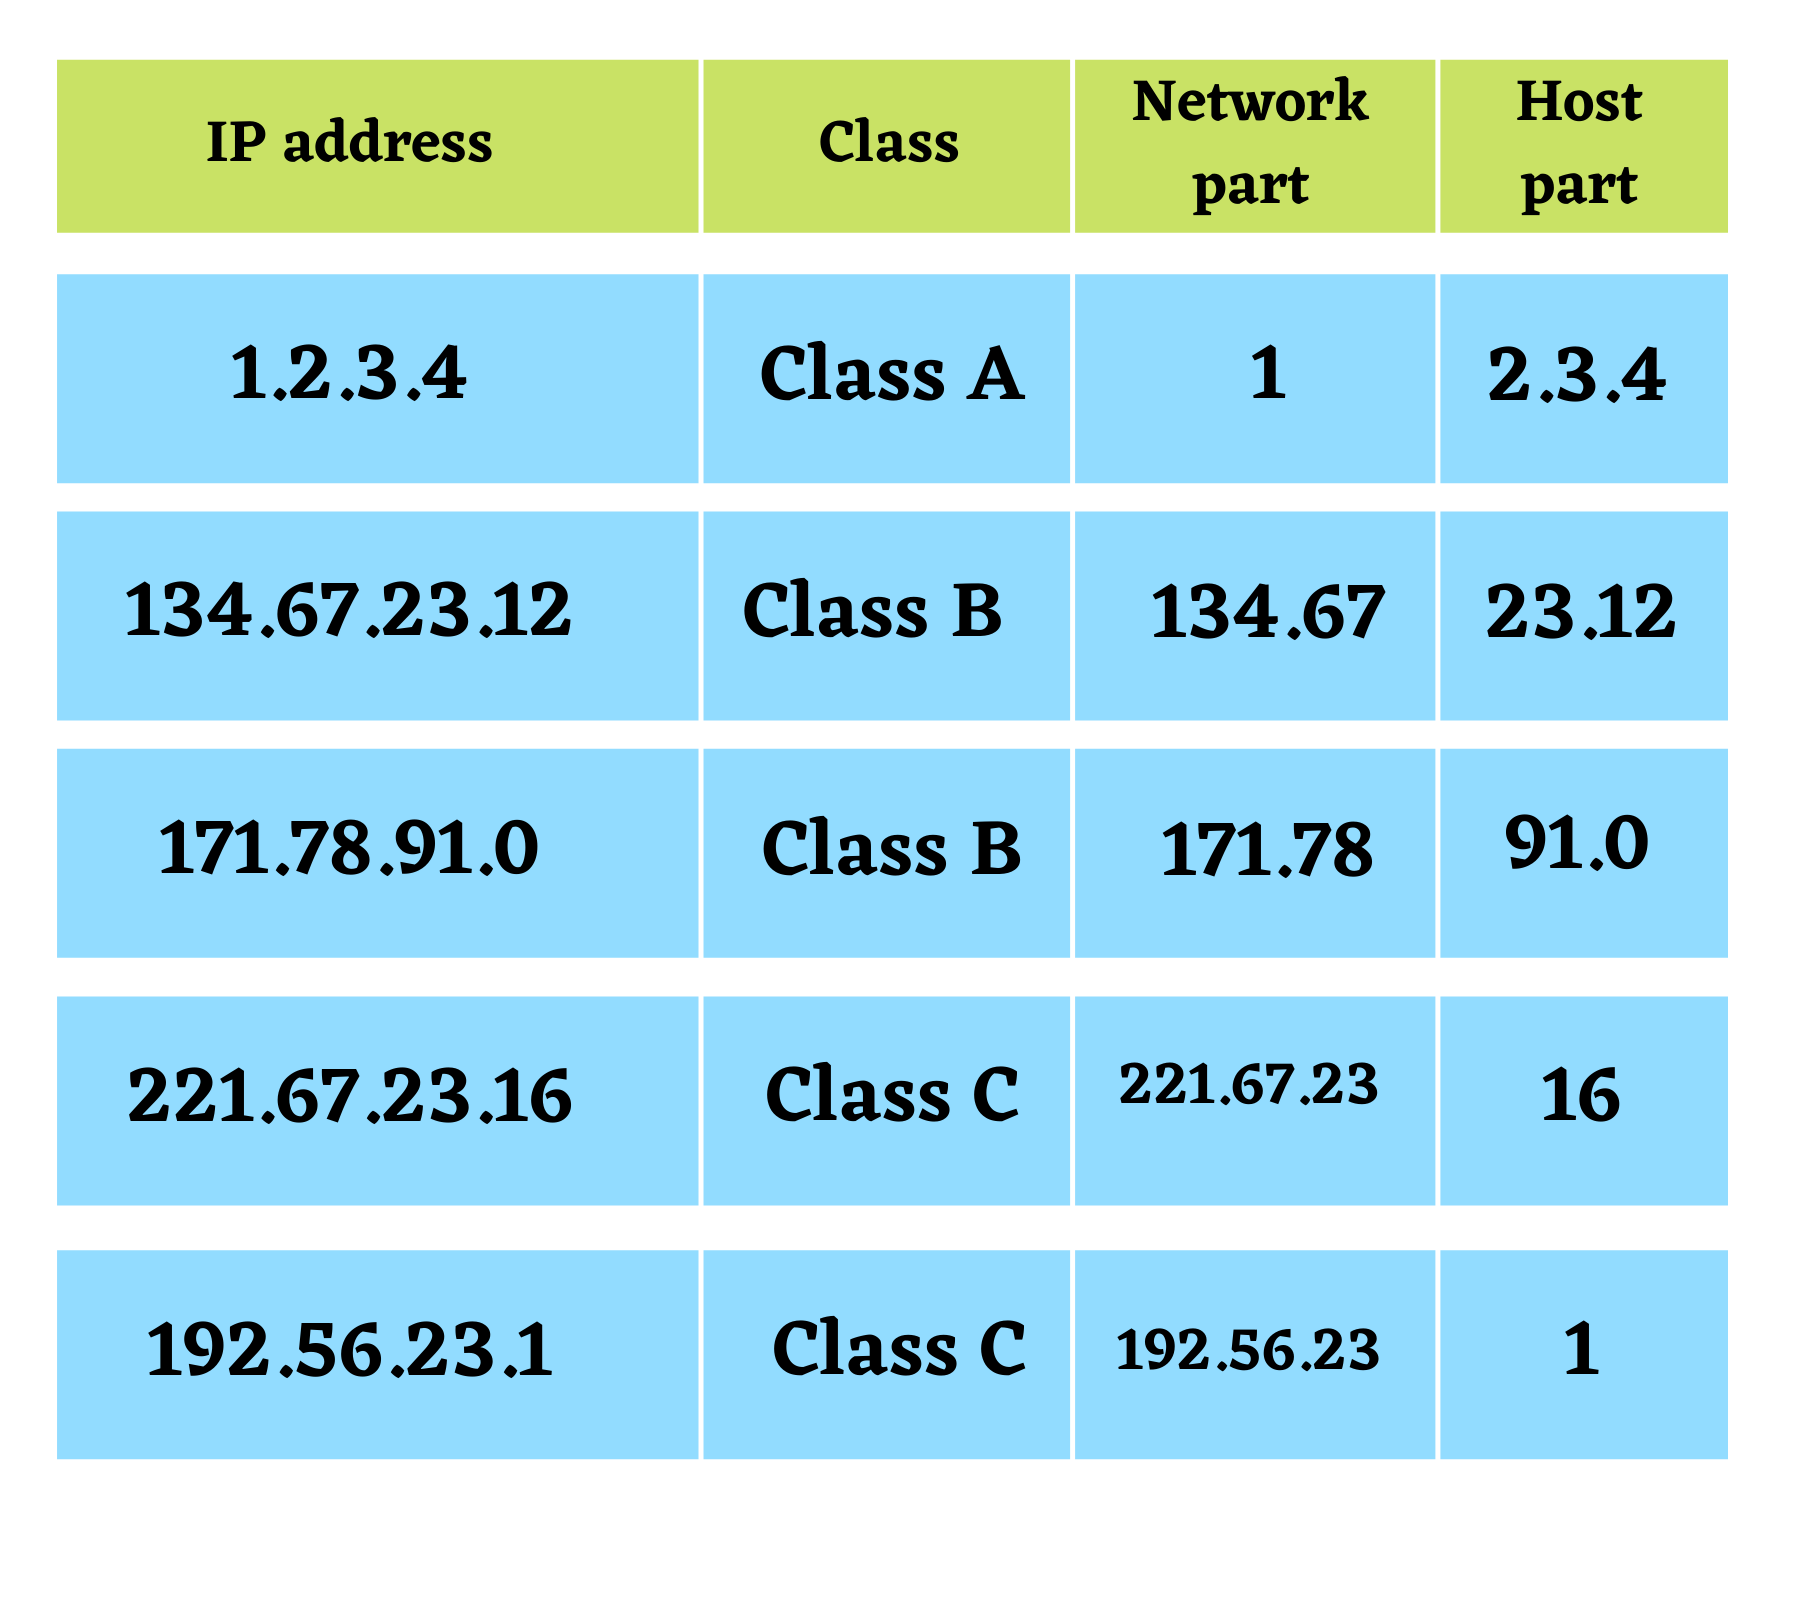
\includegraphics[scale=.3]{content/chapter14/images/ip_example.png}
	\caption{IP address classification according to class }
	\label{fig:type}
\end{figure}	




\end{flushleft}
\newpage